\section{Occupancy Grid Map prediction methods using Deep Learning} \label{sec:ogm_methods}
%% OGM Prediction
\gls{OGM} prediction is the prediction of a sequence of future \glspl{OGM} given a past sequence of \glspl{OGM}. This literature review focuses on \gls{OGM} prediction using deep learning. The goal is to train a deep learning network until it accurately generalizes traffic behavior and extrapolates that behavior to make predictions. To achieve this, first, \gls{OGM} data is required to train the network. The data, in the form of \gls{OGM} sequences, can be generated from a dataset, as is discussed in chapters \ref{sec:ogm} and \ref{sec:datasets}. Second, a suitable network architecture is required which can process \gls{OGM} sequences. The network should extract spatial and temporal features of traffic behavior to generate predictions. Third, a suitable loss function is required to evaluate the network's performance during training to update its weights. Like a metric, as discussed in chapter \ref{sec:metrics}, the loss function should ideally evaluate the predictions based on safety assurance. The chosen dataset, the network architecture, and the loss function that is used to update the network's weights all influence the prediction results. Finally, a metric is used to quantitatively evaluate different deep learning \gls{OGM} prediction methods. By comparing the metric outcomes for each method, the best performing method can be picked.  \\

This chapter gives an overview of current ego-vehicle traffic scene \gls{OGM} prediction methods. All described methods are deep learning based. First, section \ref{subsec:prednet} discussed three methods that are based on the PredNet \cite{lotter2016deep} architecture. Second, section \ref{subsec:dogma_pred} discusses two \gls{DOGMa} prediction methods. Third, section \ref{subsec:deeptrack} discusses two methods that are based on a deep tracking network architecture. Fourth, \ref{subsec:motionnet} discusses a method that is based on the MotionNet \cite{wu2020motionnet} architecture. After these methods are reviewed, the loss functions that are used to update the network's weights in each of the methods are evaluated in section \ref{subsec:lossfunc}. This chapter ends with section \ref{subsec:con_method}, which provides the answer to the final sub-question of this literature study: \airquote{\textit{What is a good Deep Learning method to generate \gls{OGM} predictions?}}


%% PredNet
\subsection{PredNet-based \gls{OGM} predictors} \label{subsec:prednet}
This section covers three methods that are all based on Lotter's \cite{lotter2016deep} Predictive Coding Network (PredNet) architecture (As is shown in figure \ref{fig:PredNet_architecture}). First, Itkina \cite{itkina2019dynamic} adjusts PredNet to be suitable for \gls{OGM} prediction. Second, Lange \cite{lange2020attention} attempts to improve Itkina's \cite{itkina2019dynamic} architecture by adding an attention mechanism that better learns dependencies between sequential grid cells. Third, Toyungyernsub \cite{toyungyernsub2020double} extends Itkina's \cite{itkina2019dynamic} architecture to separate the static from the dynamic environment so the network can better distinguish dynamic behavior.  \\

% Itkina
Initially, Itkina \cite{itkina2019dynamic} proposes to utilize PredNet, an architecture based on the human brain predictive coding principle. This principle hypothesizes that the human brain continually predicts its incoming stimuli (e.g. visual stimuli from the eyes), compares these predictions against the actual stimuli, and generates an error signal to update the predictions. To mimic this principle, the PredNet architecture consists of multiple concatenated modules that all contain the same four parts: an input layer, a representation layer, a prediction layer, and an error representation layer (See figure \ref{fig:PredNet_architecture}). The input layer obtains features from the \gls{OGM} (i.e. the actual stimulus) using convolutions and pooling. Then, a prediction of those features is made by the prediction layer (analogous to the brain's predictions), using the representation layer's features. The error representation layer generates an error by subtracting the input features from the predicted features (like the brain's generated error signal). After non-linearizing, the error is linked to both the representation layer and the output of the module. The representation layer learns temporal and spatial patterns from the error and the representation layers of neighboring modules using a \gls{ConvLSTM}. Recurrently, the prediction layer then uses the representation layer's features to make predictions of the input features. Originally, the \gls{ConvLSTM} was used for video prediction \cite{lotter2016deep}. \\

\begin{figure}[h]
	\centering
	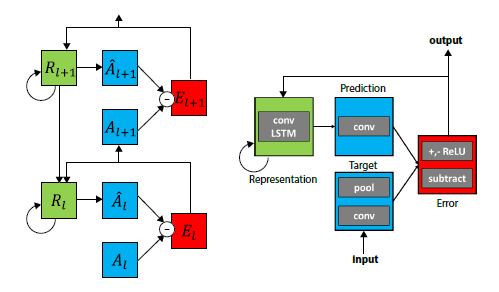
\includegraphics[width=0.8\linewidth]{Figures/Methods/PredNet_architecture}
	\caption{\airquote{Predictive Coding Network (PredNet). Left: Illustration of information flow within two layers. Each layer consists of representation neurons ($R_l$), which output a layer-specific prediction at each time step ($\hat{A_l}$), which is compared against a target ($A_l$) to produce an error term ($E_l$), which is then propagated laterally and vertically in the network. Right: Module operations for case of \gls{OGM} sequences.} \cite{lotter2016deep}.}
	\label{fig:PredNet_architecture}
\end{figure}

Itkina \cite{itkina2019dynamic} deems the network to be suitable for \gls{OGM} prediction as well because an \gls{OGM}'s format (a grid with elements ranging from $0$ to $1$) is similar to an image. Moreover, an \gls{OGM} sequence is then considered similar to a video. Therefore, Itkina \cite{itkina2019dynamic} repurposes the \gls{ConvLSTM} \cite{shi2015convolutional} for \gls{OGM} prediction. The convolutional part of the \gls{ConvLSTM} is efficient in obtaining spatial features from image-like data structures. Subsequently, the \gls{LSTM} \cite{hochreiter1997long} is a type of \gls{RNN} architecture that can process sequential data and keeps track of long-term dependencies in the features obtained from the \gls{OGM} sequences. \\

To train the PredNet, Itkina \cite{itkina2019dynamic} generates \glspl{OGM} from the \gls{KITTI} \cite{geiger2013vision} dataset. The L1-loss is used as the loss function as shown in equation \ref{eq:l1}. The L1-loss is the sum of absolute errors between the grid cells in the ground truth \gls{OGM} $I$ of size $m \times n$, and its prediction $K$, where $i, j$ are the coordinates of the \gls{OGM}. This loss function assumes an independence between grid cells. Itkina \cite{itkina2019dynamic} compares the PredNet's performance with a baseline that assumes a static environment (for the short period of time the predictions last), with an FCN network, and with a particle filter predictor. Itkina \cite{itkina2019dynamic} also compares the performance of the network with multiple variations of the input \glspl{OGM}. Using only static \glspl{OGM} is compared with using an additional \gls{DOGMa}, which includes an additional dimensional layer to the \gls{OGM} that contains dynamic state information (e.g. velocity), as discussed in chapter \ref{subsec:OGM_ext_form}. Furthermore, using \gls{DST} to generate the \glspl{OGM} is compared with using the probabilistic alternative. Comparisons are done qualitatively, by visually comparing, and with the \glsfirst{MSE} metric that compares each cell of the \glspl{OGM}.  \\

\begin{equation} \label{eq:l1}
	\text{L1-loss} = \sum_{i=0}^{m-1}\sum_{j=0}^{n-1}|I(i,j)-K(i,j)|
\end{equation}

The research of Itkina \cite{itkina2019dynamic} found that the PredNet outperforms the other investigated methods. Also, the \gls{DST}-based method performs better than the probability based method, and the difference in performance between the \gls{OGM} and the \gls{DOGMa} is almost none. For longer predictions, the objects in the \gls{OGM} become blurry or even disappear from the environment. \\

% Lange
To counter the blurriness and object disappearance for longer term predictions, Lange \cite{lange2020attention} proposes the \gls{AAConvLSTM} for environment prediction. Lange \cite{lange2020attention} stresses the importance of \gls{OGM} predictions, because this "approach facilitates the use of occupancy state estimation under uncertainty to update the belief of surroundings" \cite{lange2020attention}. However, the predictions must be reliable. Therefore, Lange \cite{lange2020attention} tries to reduce blurriness by implementing an attention mechanism into the PredNet architecture, which originated from creating long-term dependencies in language processing. Attention augmented convolutions replace the regular convolutions of the original \gls{ConvLSTM} to form the \gls{AAConvLSTM}. These attention augmented convolutions highlight inter-dependencies between spatial and temporal dimensions of the \gls{OGM} sequences. Figure \ref{fig:attention_example} shows an example of the attention mechanism applied to an image. Using attention augmented convolutions, compared to regular convolutions, allows the \gls{LSTM} to store more relevant information in its long-term memory. This, in turn, Lange \cite{lange2020attention} expects to improve the network's prediction accuracy. \\

\begin{figure}[h]
	\centering
	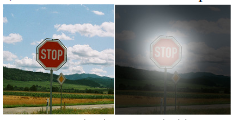
\includegraphics[width=0.7\linewidth]{Figures/Methods/Attention}
	\caption{An example of the attention mechanism applied to an image \cite{xu2015show}. The mechanism places its attention on the STOP sign as it learned that this sign is the most relevant information it should retain in its memory.}
	\label{fig:attention_example}
\end{figure}

Lange \cite{lange2020attention} trains the \gls{AAConvLSTM} PredNet using the Waymo \cite{sun2020scalability} and \gls{KITTI} \cite{geiger2013vision} datasets. The L1-loss is used as the loss function (See equation \ref{eq:l1}), which evaluates each grid cell independently. When comparing the results with using the original PredNet architecture and another baseline, the \gls{AAConvLSTM} performs better both based on qualitative visual comparison and based on the \gls{MSE} and \glsfirst{IS} metrics. However, blurriness and disappearance of objects remains. \\

% Toyungyernsub
Toyungyernsub \cite{toyungyernsub2020double} also attempts to counter the blurriness and disappearing objects that resulted from Itkina's \cite{itkina2019dynamic} method for long-term predictions. Itkina \cite{itkina2019dynamic} concluded that there was almost no difference between using an \gls{OGM} or a \gls{DOGMa} as input. However, Toyungyernsub \cite{toyungyernsub2020double} expects that incorporating dynamic information directly in the network's architecture can solve the problems of Itkina's \cite{itkina2019dynamic} network. Therefore, they propose a double-prong \gls{ConvLSTM} network based on the PredNet architecture (figure \ref{fig:double_prong} shows the network's pipeline). This network splits its architecture in static and a dynamic prong. The static prong takes as input the static \glspl{OGM} and makes static predictions, while the dynamic prong does the same for the \glspl{DOGMa}. Instead of generating \glspl{DOGMa} by using a particle filter to obtain velocity data (see chapter \ref{subsec:OGM_ext_form}), Toyungyernsub \cite{toyungyernsub2020double} uses object detection and tracking to determine each grid cell's velocity between two separate \gls{OGM} frames. Subsequently, the static and dynamic \gls{OGM} predictions are fused to form a joint prediction as the output of the network. 

\begin{figure}[h]
	\centering
	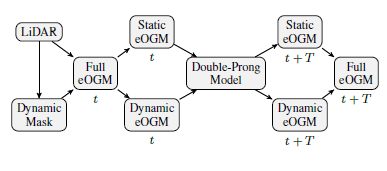
\includegraphics[width=0.7\linewidth]{Figures/Methods/Double_Prong}
	\caption{The Double-Prong network pipeline proposed by Toyungyernsub \cite{toyungyernsub2020double}. This network separately predicts the future static and dynamic \glspl{OGM} and then fuses them to create the complete \gls{OGM} prediction.}
	\label{fig:double_prong}
\end{figure}

The double-prong network is trained on the Waymo \cite{sun2020scalability} dataset and uses the L1-loss as loss function (See equation \ref{eq:l1}), which evaluates each grid cell independently. The method outperforms the original PredNet and two other baselines both in terms of the \gls{MSE} and \gls{IS} metrics and by visual comparison. The blurriness and disappearance of objects reduces significantly. For future work, incorporating multi-modality into the predictions is advised because the predicted object orientations were not always correct due to the variety of directions the objects could head for. \\


\subsection{\gls{DOGMa} predictors} \label{subsec:dogma_pred}
This section elaborates on two methods for \gls{DOGMa} prediction. First, Hoermann's \cite{hoermann2018dynamic} method is discussed which uses a \gls{CNN}. Then, Schreiber's \cite{schreiber2019long} method is discussed, which builds upon Hoermann's \cite{hoermann2018dynamic} research and uses encoder-decoder \glspl{ConvLSTM} instead of a \gls{CNN}. \\

Hoermann \cite{hoermann2018dynamic} proposes to predict \glsfirst{DOGMa} using a \glsfirst{CNN}. The network requires one \gls{DOGMa} of the current time step and predicts up to $3$ seconds into the future with time steps of $0.5$ seconds. Only one input \gls{DOGMa} is used because it is hypothesized that most information necessary for prediction can be found in the dynamic representation and the relation between the cells and not necessarily from the past \glspl{DOGMa}. Then, about $0.25\%$ of a \gls{DOGMa} contains dynamic grid cells, so if the network falsely predicts dynamic grid cells, the resulting loss would be marginally affected. Therefore, the network learns to segment static and dynamic parts of the \gls{DOGMa}. This is done, so that the loss can be split up into a static loss and a dynamic loss. By weighing dynamic grid cells relatively more than static grid cells in the loss, the network is prevented from ignoring the dynamic grid cells in its predictions. The output of the network is a multichannel \gls{OGM} with one channel containing the occupancy of static grid cells and several channels, for each predicted time step one, containing the future occupancy of dynamic grid cells. The network's architecture is a downscaling cascade of \glspl{CNN} followed by upscaling deconvolutions. It is based on Noh's \cite{noh2015learning} semantic segmentation network (See figure \ref{fig:cnn_hoermann}) but it replaces the unpooling layers with deconvolutions. This is because deconvolution kernels can be learned which allows for more parameters to generate predictions.  \\

\begin{figure}[h]
	\centering
	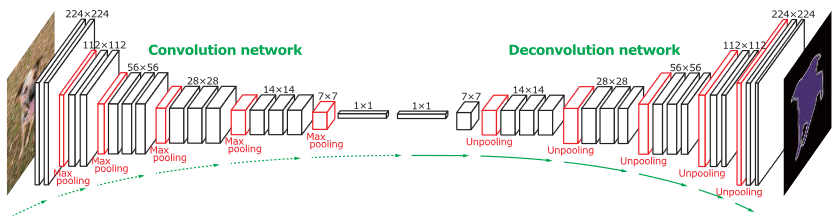
\includegraphics[width=0.8\linewidth]{Figures/Methods/Hoermann_CNN}
	\caption{Noh's \cite{noh2015learning} \gls{CNN} architecture that forms the basis for Hoermann's \cite{hoermann2018dynamic} \gls{DOGMa} prediction network. In Hoermann's \cite{hoermann2018dynamic} architecture, the unpooling layers are replaced by deconvolution layers.}
	\label{fig:cnn_hoermann}
\end{figure}

Hoermann's \cite{hoermann2018dynamic} network is trained on their own recorded dataset. The \gls{MSE} is used as loss function (See equation \ref{eq:mse} in chapter \ref{sec:metrics}), in which the loss is subdivided into weighed static and dynamic parts. This loss assumes independent grid cells. The results are evaluated against a particle filter baseline using the \glsfirst{TPR},\glsfirst{FPR}, and \glsfirst{ROC} as metrics and by visual comparison. The evaluations shows that the proposed method is better than a particle filter baseline. The proposed method performs multimodal predictions, can distinguish static from dynamic objects, and provides more accurate predictions than the particle filter. This is because the convolutional layers capture the DOGMa's cell dependencies where particle filters assume independent cells. However, due to uncertainty longer term predictions become vaguer. \\

Schreiber \cite{schreiber2019long} builds upon Hoermann's \cite{hoermann2018dynamic} research by expanding the \gls{CNN} with a \gls{ConvLSTM} encoder and decoder containing \glspl{ConvLSTM} and with \gls{ConvLSTM} skip-connections between the down-scaling and up-scaling parts of the network (See figure \ref{fig:convlstm_schreiber}). The \glspl{ConvLSTM} in the encoder and decoder capture spatial and temporal correlations. The skip-connections convey high resolution features, including occluded objects, to the up-scaling layers. Like Hoermann's \cite{hoermann2018dynamic} network, Schreiber's \cite{schreiber2019long} network also splits the static and dynamic predictions to compute the loss separately. The network outputs a multi-channel \gls{OGM}. One channel contains the occupancy of static grid cells, and for every predicted time step there are channels with the occupancy of the dynamic grid cells. \\

\begin{figure}[h]
	\centering
	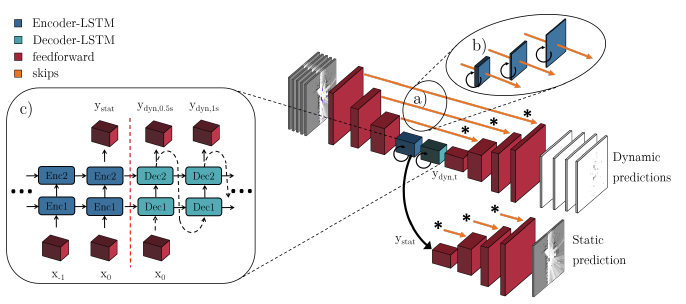
\includegraphics[width=0.8\linewidth]{Figures/Methods/Schreiber_ConvLSTM}
	\caption{Schreiber's \cite{schreiber2019long} \gls{ConvLSTM} encoder-decoder network with \gls{ConvLSTM} skip connections.}
	\label{fig:convlstm_schreiber}
\end{figure}

To train the network, Schreiber \cite{schreiber2019long} recorded their own dataset. The loss function for the static environment is the L1-score (equation \ref{eq:l1}) and the \gls{MSE} (equation \ref{eq:mse} in chapter \ref{sec:metrics}) for the dynamic environment. Both loss functions evaluate each grid cell independently. The F1-score and the \gls{ROC} are used as metric to compare Schreiber's \cite{schreiber2019long} network with Hoermann's \cite{hoermann2018dynamic} network, Dequaire's \cite{dequaire2018deep} network (which is discussed in the following section), and a particle filter. The methods are also compared based on visual quality. Schreiber's \cite{schreiber2019long} method shows better F1-score results and better qualitative results compared to Hoermann's \cite{hoermann2018dynamic} previous research. The static predictions remain sharp for long term predictions, even for parts of the environment that became partially occluded in the input sequence. Partially occluded dynamic obstacles are predicted accurately as well and there is multimodality in the predictions. However, the data is only recorded in a stationary scenario. Therefore, the performance of the network with egomotion should researched in the future to investigate the accuracy of the predictions in driving scenarios.   

%%% Dequaire and Mohajerin
\subsection{Deep tracking based \gls{OGM} predictors} \label{subsec:deeptrack}
In this section, two \gls{OGM} prediction methods are described that use deep tracking based network architectures. First, Dequaire's \cite{dequaire2018deep} method is discussed which bases its network's architecture on the Deep Tracking framework introduced by Ondruska \cite{ondruska2016deep}. Then, Mohajerin's \cite{mohajerin2019multi} method is discussed which builds upon Dequaire's \cite{dequaire2018deep} research by implementing a difference learning architecture. \\

Dequaire's \cite{dequaire2018deep} main research problem is to uncover the true, unoccluded state of the world in terms of \glspl{OGM}, given a sequence of partially observable \glspl{OGM}. Dequaire \cite{dequaire2018deep} generates two-channel \glspl{OGM}. One channel contains the occupancy data ($0$ for Empty, $1$ for Occupied), the other channel contains visibility information ($0$ for occluded, $1$ for unoccluded). By uncovering the unoccluded state of a partially observable \gls{OGM}, tracking (partially) occluded objects through the \gls{OGM} sequence can be done more accurately. Furthermore, Dequaire \cite{dequaire2018deep} argues that \gls{OGM} prediction is the same as uncovering the unoccluded state of a completely occluded \gls{OGM}, given the past sequences of \glspl{OGM}. Besides tracking and prediction, Dequaire \cite{dequaire2018deep} also assumes that if a network learns to predict traffic behavior, it must learn to distinguish shapes and motion patterns of the observed traffic participants. With this knowledge, the network can also be trained to perform semantic segmentation if class labels are provided in the \glspl{OGM} during network training. This is because different object classes (i.e. pedestrians, cyclists, vehicles) have distinct shapes and motion patterns. To perform the tasks of tracking, prediction, and semantic segmentation, Dequaire \cite{dequaire2018deep} proposes a network based on Ondruska's \cite{ondruska2016deep} recurrent deep tracking network which contains \glspl{RNN}. However, to improve this network's memory Dequaire \cite{dequaire2018deep} uses the \glsfirst{GRU} in their network architecture (See figure \ref{fig:gru_dequaire}). A \gls{GRU} is similar to an \gls{LSTM} in that it retains memory for a longer term compared to an \gls{RNN}. However, the \gls{GRU} has fewer parameters than the \gls{LSTM}, which makes it more efficient and more suitable for training on small datasets compared to the \gls{LSTM}. Furthermore, to compensate for the ego-motion in between an \gls{OGM} sequence's time steps, Dequaire \cite{dequaire2018deep} implements a \gls{STM}. The \gls{STM} is a learnable module that uses odometry data to translate the \gls{GRU}'s hidden state of the previous time step to the current time step. \\

\begin{figure}[h]
	\centering
	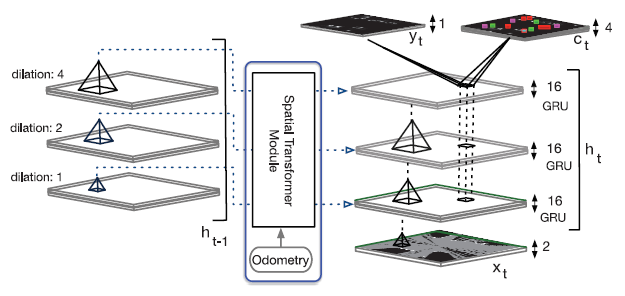
\includegraphics[width=0.8\linewidth]{Figures/Methods/Dequaire_GRU}
	\caption{Dequaire's \cite{dequaire2018deep} \gls{GRU}-based \gls{OGM} prediction network architecture. The latent features from the previous time step go through the \glsfirst{STM} to compensate for the ego-motion in between the \gls{OGM} frames.}
	\label{fig:gru_dequaire}
\end{figure}

\begin{equation} \label{eq:cross-entropy}
	\text{Cross-Entropy loss} = -\frac{1}{mn}\sum_{i=0}^{m-1}\sum_{j=0}^{n-1}(I(i,j)\cdot log(p(K(i,j)))-(1-I(i,j))\cdot log(1-p(K(i,j)))
\end{equation}

The network is trained on Dequaire's \cite{dequaire2018deep} self-recorded dataset. The traffic scenes in the dataset are in no point in time fully observable. Therefore, the network is only trained to correctly predict the occupancy of \gls{OGM}'s occluded states that are visible in future ground truth \glspl{OGM}. This is because, predictions cannot be evaluated if the ground truth does not contain visible data of the predicted content. The loss function that is used to train the network's predictions is the (binary) cross-entropy loss (equation \ref{eq:cross-entropy}). The cross-entropy loss compares the rounded values ($0$ or $1$) of grid cells in the ground truth \gls{OGM} $I$ of size $m \times n$ with the predicted occupancy probabilities of $K$, where $i, j$ are the coordinates of the \gls{OGM}. The loss increases logarithmically with the error. This loss function assumes an independence between grid cells. The prediction results are compared against Ondruska's \cite{ondruska2016deep} Deep Tracking network using the F1-score and by visual comparison. The results show that Dequaire's \cite{dequaire2018deep} \gls{GRU}-based network performs better than Ondruska's \cite{ondruska2016deep} Deep Tracking network.  \\  

Mohajerin \cite{mohajerin2019multi} builds upon Dequaire's \cite{dequaire2018deep} research and proposes a difference learning method for the prediction of \glspl{OGM} using \glspl{ConvLSTM} in the network architecture. Figure \ref{fig:diff_learn} shows the difference learning architecture. The suggested method learns the difference between consecutive \glspl{OGM} using a \gls{MFE} algorithm. The output of the \gls{MFE} algorithm is a tensor of the same height and width as the \glspl{OGM} which contains movement information in X and Y directions for each grid cell. This information is encoded and added to the encoded representation of the input \gls{OGM} in the network's architecture. Subsequently, the encoded \gls{OGM} and movement information flows through a \gls{ConvLSTM} core after which it is decoded and results in the predicted change of motion for each grid cell of the \gls{OGM}. This predicted change of motion is added to the input \gls{OGM} and processed by a feed-forward classifier layer that provides the prediction of the full \gls{OGM} for one time step. This predicted \gls{OGM} is inserted back into the network to predict the next time step. This is iterated for the number of predicted time steps that are desired. \\

\begin{figure}[h]
	\centering
	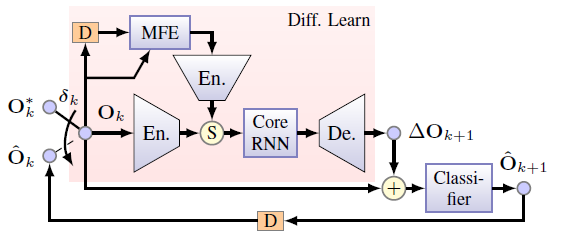
\includegraphics[width=0.6\linewidth]{Figures/Methods/Difference_Learning}
	\caption{Mohajerin's \cite{mohajerin2019multi} \gls{ConvLSTM}-based difference learning \gls{OGM} prediction network architecture. Two consecutive \glspl{OGM} go through the \gls{MFE} module to obtain a movement information for each grid cell. The encoded movement information is added to the current encoded \gls{OGM} and processed by the Core \gls{RNN} (the \gls{ConvLSTM}). After decoding the result, it is processed by the Classifier to predict an \gls{OGM} for one time step. To predict the next time step, the predicted \gls{OGM} is inserted as the new input of the network.}
	\label{fig:diff_learn}
\end{figure}

\begin{equation} \label{eq:l2}
	\text{L2-loss} = \sum_{i=0}^{m-1}\sum_{j=0}^{n-1}(I(i,j)-K(i,j))^2
\end{equation}

The network is trained on the \gls{KITTI} \cite{geiger2013vision} dataset. A summation of three loss functions is used to train the network: the cross-entropy loss (equation \ref{eq:cross-entropy}), the L2-loss (equation \ref{eq:l2}), and the \gls{SSIM} (equation \ref{eq:ssim} in chapter \ref{sec:metrics}). The L2-loss is the sum of squared errors between the grid cells in the ground truth \gls{OGM} $I$ of size $m \times n$, and its prediction $K$, where $i, j$ are the coordinates of the \gls{OGM}. The cross-entropy loss and the L2-loss assume an independence between grid cells. However, the \gls{SSIM} loss evaluates the structures between grid cells and thus considers the dependencies between grid cells. Mohajerin's \cite{mohajerin2019multi} network is compared to a close approximation of Dequaire's \cite{dequaire2018deep} network using the \gls{TPR}, \gls{TNR}, and the \gls{SSIM} metrics. 
The difference learning architecture outperforms Dequaire's \cite{dequaire2018deep} architecture in predicting future \glspl{OGM} based on the \glspl{SSIM}. Mohajerin \cite{mohajerin2019multi} mentions that the provided ground truth data (from the \gls{KITTI} \cite{geiger2013vision} dataset) is an inadequate target to which the predictions should be compared, since the ground truth only contains the visible borders within the \gls{AV}'s FOV, while the model predicts the whole environment. As a result, the network can accurately predict occupied cells outside the FOV of the ground truth data which is then erroneously considered a false positive because the GT data is not complete.

%%% MotionNet
\subsection{MotionNet multi-channel \gls{OGM} predictor} \label{subsec:motionnet}
This last section discusses Wu's \cite{wu2020motionnet} MotionNet \gls{OGM} prediction method. Wu \cite{wu2020motionnet} performs perception and motion prediction with 3D LiDAR data as input. A sequence of LiDAR sweep 3D point clouds synchronized to the current time frame is converted to \gls{BEV} maps by voxellizing the point cloud and representing it as a 2D pseudo-image where the height dimension corresponds to the image channels. So, it is similar to having a multi-channel \gls{OGM} where each channel represents a different height in the environment. This representation makes convolution possible. The MotionNet is a spatio-temporal pyramid network (See figure \ref{fig:spatiotemporal}). It contains an encoder with multiple \gls{STC} blocks that consist of standard 2D convolutions for capturing spatial features, followed by a 1D convolution. The encoder is followed by a decoder using deconvolutions. Between the encoder and decoder there are temporal pooling skip-connections that convey temporal features at different scales to retain both global and local spatio-temporal contexts. The network contains three output heads each providing an output with specific information. The first head provides semantic segmentation of the \gls{OGM}. The second head provides an \gls{OGM} prediction for $N$ time steps. The third head provides a classification of whether a grid cell is dynamic or static. Together, the three heads from a multi-channel \gls{OGM} output with object labels, predictions, and dynamic information. This is similar to a sequences of \glspl{DOGMa} with semantic information. \\


\begin{figure}[h]
	\centering
	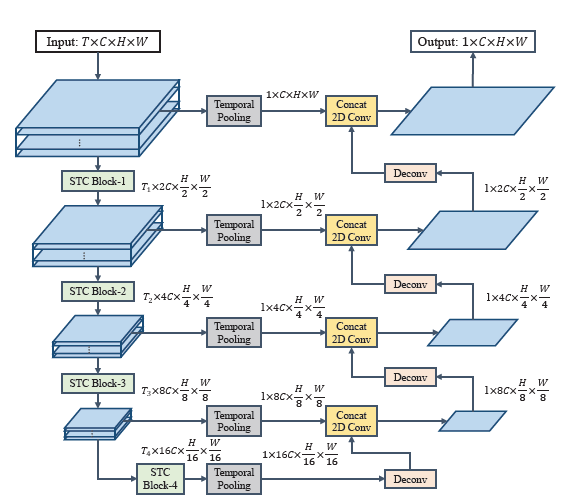
\includegraphics[width=0.6\linewidth]{Figures/Methods/STC_Block}
	\caption{MotionNet, Wu's \cite{wu2020motionnet} spatio-temporal pyramid network containing \gls{STC} building blocks and temporal pooling skip connections to predict \glspl{OGM}.}
	\label{fig:spatiotemporal}
\end{figure}
%TODO: loss function here is rewritten and extended
The network is trained on the Nuscenes \cite{caesar2020nuscenes} dataset. The loss functions that are used are the L1-loss (equation \ref{eq:l1}) for the predictions, and the cross-entropy loss (equation \ref{eq:cross-entropy}) for the dynamic and semantic information. Both loss functions assume independence between grid cells. However, to compensate for this assumption, \cite{wu2020motionnet} computes three additional losses. These losses are based on the assumptions that an object's grid cells move equally and with minimal dynamic changes per time step, and that the background remains static. The first two are the spatial and foreground temporal consistency losses. These losses minimize the motion between the grid cells corresponding to a single object, and the average motion of a single object's grid cells through time respectively, in the predictions. The third loss is the background temporal consistency loss and minimizes the movement of grid cells that do not belong to any annotated objects in the predictions. The three losses are all based on the L1-loss, but by using semantic information to evaluate objects (i.e. clusters of grid cells between which dependency is assumed), these losses do consider grid cell dependencies. \cite{wu2020motionnet} concludes that after implementing these losses, the predictions became smoother. However, relations between individual objects are still not considered in the loss functions. \\

The MotionNet network \cite{wu2020motionnet} is compared with Schreiber's \cite{schreiber2019long} \gls{ConvLSTM} encoder-decoder network, and four other baselines. The \gls{MSE} metric and \gls{MeSE} metric (the median value of the squared errors of the \gls{OGM}'s cells) are used for evaluation. The evaluation is done by comparing the results at different velocities of the grid cell dynamics: at $0 m/s$, $\leq 5 m/s$, and $> 5 m/s$. Wu's \cite{wu2020motionnet} MotionNet outperforms the other networks especially because of its ability to distinguish static and dynamic obstacles well.  

\subsection{Loss Functions} \label{subsec:lossfunc}
In the previous sections, several loss functions were used to train the deep learning networks. The loss function that is used influences what errors are penalized and thus how a network's weights are updated. The loss functions, similarly to metrics, evaluate the resemblance between a ground truth \gls{OGM} and its prediction. So, the better a loss function can determine the quality of a prediction, the more accurate the weights of a network can be updated to achieve accurate predictions. Therefore, this section evaluates the loss functions that are used in the previous sections. Since metrics and loss functions fulfill the same purpose, the criteria to evaluate the metrics are also used to evaluate the loss functions. An additional criterion for loss functions is that they must be differentiable to backpropagate the error through the deep learning network. However, in this case, all loss functions are differentiable since they have been used in the networks described earlier in this chapter. Table \ref{tab:loss_func} shows how well the loss functions meet the criteria. The criteria are listed below the table. Because all loss functions except the \gls{SSIM} assume an independence between the grid cells of the \gls{OGM} (or independence between detected objects within the \gls{OGM}), they only meet the first criterion. The \gls{SSIM} does consider dependencies between grid cells, since it evaluates the similarity of grid cell structures. Therefore, as discussed in chapter \ref{sec:metrics}, the \gls{SSIM} meets all criteria. 

\begin{table}
	\centering
	\resizebox{0.5\linewidth}{!}{%
		\begin{tabular}{lccccc} 
			\toprule
		& \textbf{L1} & \textbf{L2} & \textbf{\gls{MSE}} & \textbf{Cross-Entropy} & \textbf{\gls{SSIM}} \\ 
			\midrule
			\textbf{1.} & \textbf{\cmark} & \textbf{\cmark} & \textbf{\cmark} & \textbf{\cmark} & \textbf{\cmark} \\
			\textbf{2. } & \textbf{\xmark} & \textbf{\xmark} & \textbf{\xmark} & \textbf{\xmark} & \textbf{\cmark} \\
			\textbf{3. } & \textbf{\xmark} & \textbf{\xmark} & \textbf{\xmark} & \textbf{\xmark} & \textbf{\cmark} \\
			\textbf{4. } & \textbf{\xmark}& \textbf{\xmark} & \textbf{\xmark} & \textbf{\xmark} & \textbf{\cmark} \\
			\textbf{5.} & \textbf{\xmark} & \textbf{\xmark} & \textbf{\xmark} & \textbf{\xmark} & \textbf{\cmark} \\
			\bottomrule
		\end{tabular}
	}
	\caption{An overview of the loss functions that are used in the \gls{OGM} prediction methods. For each criterion (numbers 1 to 5), the table shows whether the loss function meets it (\textbf{\cmark}) or not (\textbf{\xmark}). The criteria are as follows (the same criteria as the metrics criteria from chapter \ref{sec:metrics}). 
		\\\hspace{\textwidth} 
		\textbf{1.} The loss function considers the whole \gls{OGM} in its evaluation.
		\textbf{2.} The loss function weighs local deletion or addition errors more than global noise errors.
		\textbf{3.} The loss function weighs big displacement errors more than small displacement errors.
		\textbf{4.} The loss function weighs errors close to the \gls{AV} (often the center of the \gls{OGM}) more than errors further from the \gls{AV}.
		\textbf{5.} The loss function weighs additions and deletions more than displacements.
	}
	\label{tab:loss_func}
\end{table} 

\subsection{What is a good Deep Learning method to generate \gls{OGM} predictions?} \label{subsec:con_method}
The best results of each method that is described in this chapter are shown in table \ref{tab:method_results}. Also, table \ref{tab:method_overview} shows an overview of the \gls{OGM} prediction methods. Since not all methods are trained on the same datasets and evaluated using the same metrics, it is difficult to compare them. Even within the same method's subcategories (PredNet, \gls{DOGMa} prediction, Deep Tracking, and MotionNet) there is no consistent use of datasets and metrics. If the use of different datasets is not considered, \cite{lange2020attention} provides the lowest \gls{MSE} and the lowest \gls{IS} (on the Waymo \cite{sun2020scalability} dataset), given the available information. Furthermore, Mohajerin's \cite{mohajerin2019multi} method has the highest \gls{TPR}. Then, when looking at the \gls{ROC} curves that compare Schreiber's method \cite{schreiber2019long} with Hoermann's method \cite{hoermann2018dynamic} in figure \ref{fig:roc_schreiber}, Schreiber's method \cite{schreiber2019long} performs better. Also, Schreiber's method \cite{schreiber2019long} has the highest F1-score. Unfortunately, Mohajerin's \cite{mohajerin2019multi} \gls{SSIM} score cannot be compared because no other methods are evaluated using that metric. After this analysis, still no conclusive answer can be given about what \gls{OGM} generation method is considered good or better than the other investigated ones. Especially since chapter \ref{sec:metrics} concludes that the \gls{SSIM} and \gls{IS} metrics are more suitable to evaluate \glspl{OGM} compared to the other metrics. This makes it hard to determine how much weight a result from a specific metric should be given compared to the other metrics. Therefore, comparing the methods using different metrics is not feasible. In conclusion, to answer the question: \airquote{\textit{What is a good Deep Learning method to generate \gls{OGM} predictions?}}, the different methods should be evaluated using the same (suitable) metric(s). 

\begin{table}[h!]
	\centering
	\resizebox{\linewidth}{!}{%
		\begin{tabular}{llm{10em}llm{10em}l} 
			\toprule
			\textbf{Paper/Method} & \textbf{Dataset(s)} & \textbf{Network(s)} & \textbf{Input} & \textbf{Output} & \textbf{Loss Function(s)} & \textbf{Metric(s)} \\ 
			\midrule
			\textbf{Itkina \cite{itkina2019dynamic}} & KITTI \cite{geiger2012we} & PredNet-based \newline ConvLSTM & DOGMa, DST OGM & DST OGM & L1-Loss & MSE \\
			\textbf{Lange \cite{lange2020attention}} & KITTI \cite{geiger2012we}, Waymo
			\cite{sun2020scalability} & PredNet-based \newline AAConvLSTM & DST OGM & DST OGM & L1-Loss & MSE, IS \\
			\textbf{Toyungyernsub \cite{toyungyernsub2020double}} & Waymo \cite{sun2020scalability} & PredNet-based \newline ConvLSTM \newline
			Double-Prong & DOGMa, DST OGM & DST OGM & L1-Loss & MSE, IS \\
			\textbf{Hoermann \cite{hoermann2018dynamic}} & Own & CNN-based & DOGMa & OGM & MSE & ROC, TPR, FPR \\
			\textbf{Schreiber \cite{schreiber2019long}} & Own  & Grid Predictor Model
			ConvLSTM-Encoder-Decoder & DOGMa & OGM & L1-Loss, MSE & ROC, F1-score \\
			\textbf{Dequaire \cite{dequaire2018deep}} & Own  & Convolutional GRU & OGM with semantics & OGM with semantics & Cross-entropy~ & F1-score \\
			\textbf{Mohajerin \cite{mohajerin2019multi}} & KITTI \cite{geiger2012we} & ConvLSTM-Encoder-Decoder-based \newline
			variations & OGM & OGM & Cross-entropy, \newline L2-Loss, SSIM & TPR, TNR, SSIM \\
			\textbf{Wu \cite{wu2020motionnet}} & NuScenes \cite{caesar2020nuscenes} & MotionNet CNN-based & OGM at multiple heights & DOGMa with semantics & L1-Loss, Cross-entropy & MSE, MeSE \\
			\bottomrule
		\end{tabular}
	}
	\caption{An overview of properties of the different \gls{OGM} prediction methods. }
	\label{tab:method_overview}
\end{table}

\begin{figure}[h]
	\centering
	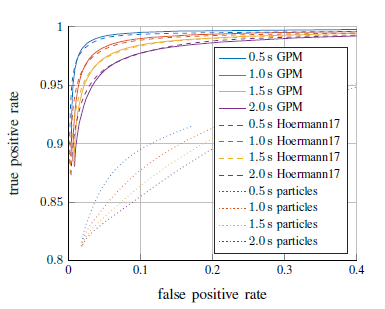
\includegraphics[width=0.5\linewidth]{Figures/Methods/ROC_schreiber}
	\caption{The \gls{ROC} curves of Schreiber's method \cite{schreiber2019long} (GPM), compared to Hoermann's method \cite{hoermann2018dynamic} and a particle filter.}
	\label{fig:roc_schreiber}
\end{figure}

\begin{table}[H]
	\centering
	\resizebox{\linewidth}{!}{
		\begin{tabular}{lp{50mm}lp{45mm}p{45mm}p{45mm}lp{45mm}l} 
			&  &  & \multicolumn{6}{c}{\textbf{Results}} \\ 
			\cmidrule{4-9}
			& \textbf{Paper/Method} & \textbf{Datasets} & \textbf{MSE ($\cdot 10^{-2}$)} & \textbf{IS} & \textbf{TPR} & \textbf{ROC} & \textbf{F1-Score} & \textbf{SSIM} \\ 
			\midrule
			\multirow{3}{*}{\rotatebox[origin=c]{90}{PredNet}} & \textbf{Itkina \cite{itkina2019dynamic}} & KITTI \cite{geiger2012we} & 3.295 ± 0.1625 & \textbf{\xmark} & \textbf{\xmark} & \textbf{\xmark} & \textbf{\xmark} & \textbf{\xmark} \\
			& \textbf{Lange \cite{lange2020attention}} & KITTI \cite{geiger2012we}, \newline Waymo
			\cite{sun2020scalability} & KITTI: 3.62 ± 0.0012, \textbf{Waymo: 2.33
			± 0.0063} & KITTI: 6.91 ± 0.06, \textbf{Waymo: 3.51 ±
			0.04} & \textbf{\xmark} & \textbf{\xmark} & \textbf{\xmark} & \textbf{\xmark} \\
			& \textbf{Toyungyernsub \cite{toyungyernsub2020double}} & Waymo \cite{sun2020scalability} & 3.17 ± 0.0007 & 5.86 ± 0.058 & \textbf{\xmark} & \textbf{\xmark} & \textbf{\xmark} & \textbf{\xmark} \\
			\multirow{2}{*}{\rotatebox[origin=c]{90}{\gls{DOGMa}}} & \textbf{Hoermann \cite{hoermann2018dynamic}} & Own & \textbf{\xmark} & \textbf{\xmark} & Min: 0.75 (0.5s), \newline Max: 0.81 (2.0s) & \textbf{\cmark} & \textbf{\xmark} & \textbf{\xmark} \\
			& \textbf{Schreiber \cite{schreiber2019long}} & Own, Nuscenes \cite{caesar2020nuscenes} & Nuscenes: 5.92 \tablefootnote{This is the weighted average \gls{MSE} based on \cite{hoermann2018dynamic}'s finding that 0.25\% of an \gls{OGM} consists of dynamic grid cells. The assumption is made that the number of grid cells with the velocities of $≤ 5 m/s$ and $> 5 m/s$ are of equal amount.}
			\cite{wu2020motionnet} &  &  & \textbf{\cmark} & \textbf{Best: 0.9 (0.5s)}, \newline \textbf{Worst: 0.8
			(2.0s)} & \textbf{\xmark} \\
			\multirow{2}{*}{\rotatebox[origin=c]{90}{\makecell[b]{Deep \\ Tracking}}} & \textbf{Dequaire \cite{dequaire2018deep}} & Own & \textbf{\xmark} & \textbf{\xmark} & \textbf{\xmark} & \textbf{\xmark} & \cite{schreiber2019long}'s
			dataset: \newline Best: 0.8 (0.5s), \newline Worst: 0.6 (1.5s)
			\cite{schreiber2019long} & \textbf{\xmark} \\
			& \textbf{Mohajerin \cite{mohajerin2019multi}} & KITTI \cite{geiger2012we} & \textbf{\xmark} & \textbf{\xmark} & \textbf{0.8836} \newline for TNR of 0.9928 & \textbf{\xmark} & \textbf{\xmark} & \textbf{0.9841} \\
			\multirow{1}{*}{\rotatebox[origin=c]{90}{\makecell[b]{Motion \\ Net}}} & \textbf{Wu \cite{wu2020motionnet}} \newline \newline & NuScenes \cite{caesar2020nuscenes} & 3.42 \tablefootnote{This is the weighted average \gls{MSE} based on \cite{hoermann2018dynamic}'s finding that 0.25\% of an \gls{OGM} consists of dynamic grid cells. The assumption is made that the number of grid cells with the velocities of $≤ 5 m/s$ and $> 5 m/s$ are of equal amount.} & \textbf{\xmark} & \textbf{\xmark} & \textbf{\xmark} & \textbf{\xmark} & \textbf{\xmark} \\ 
			\bottomrule
			\end{tabular}
		}
		\caption{The results for each \gls{OGM} prediction method categorized by the metric(s) that is/are used to evaluate the method. Some methods are trained multiple times using different datasets. In that case, the datasets are mentioned before each result.}
		\label{tab:method_results}
\end{table}

